% $Id: Note_ResFit_QCDMC_Extrapolation.tex,v 1.6 2010/07/13 17:26:14 mschrode Exp $



\begin{figure}[ht]
  \centering
    \begin{tabular}{ccc}
      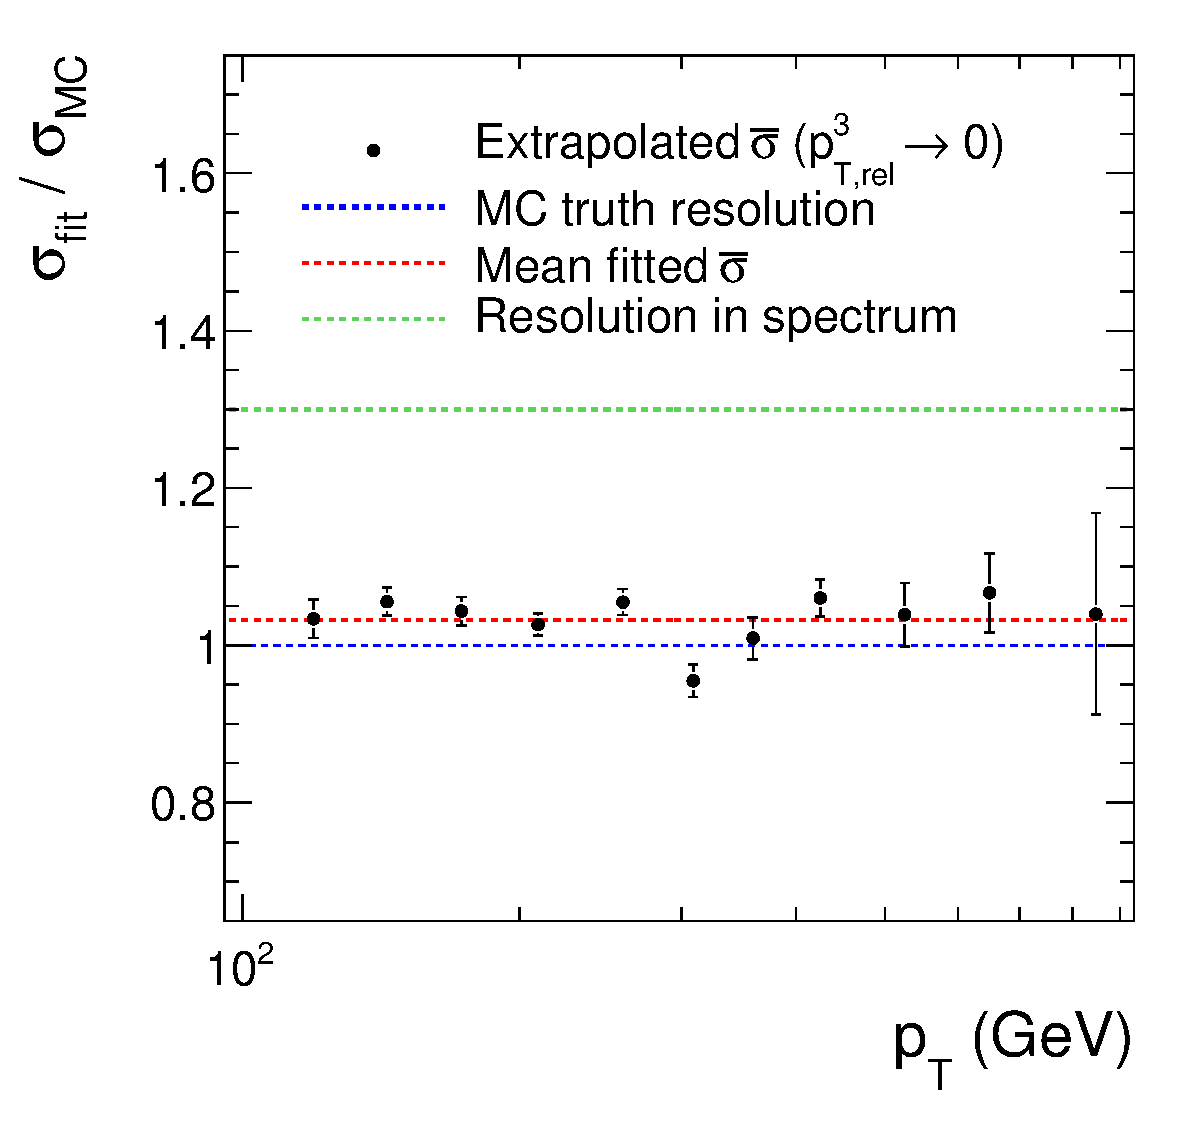
\includegraphics[width=0.3\textwidth]{figures/ResFit_Spring10QCDFlat_GaussUp30It0_Eta0_ExtrapolatedResolutionRatio} &
      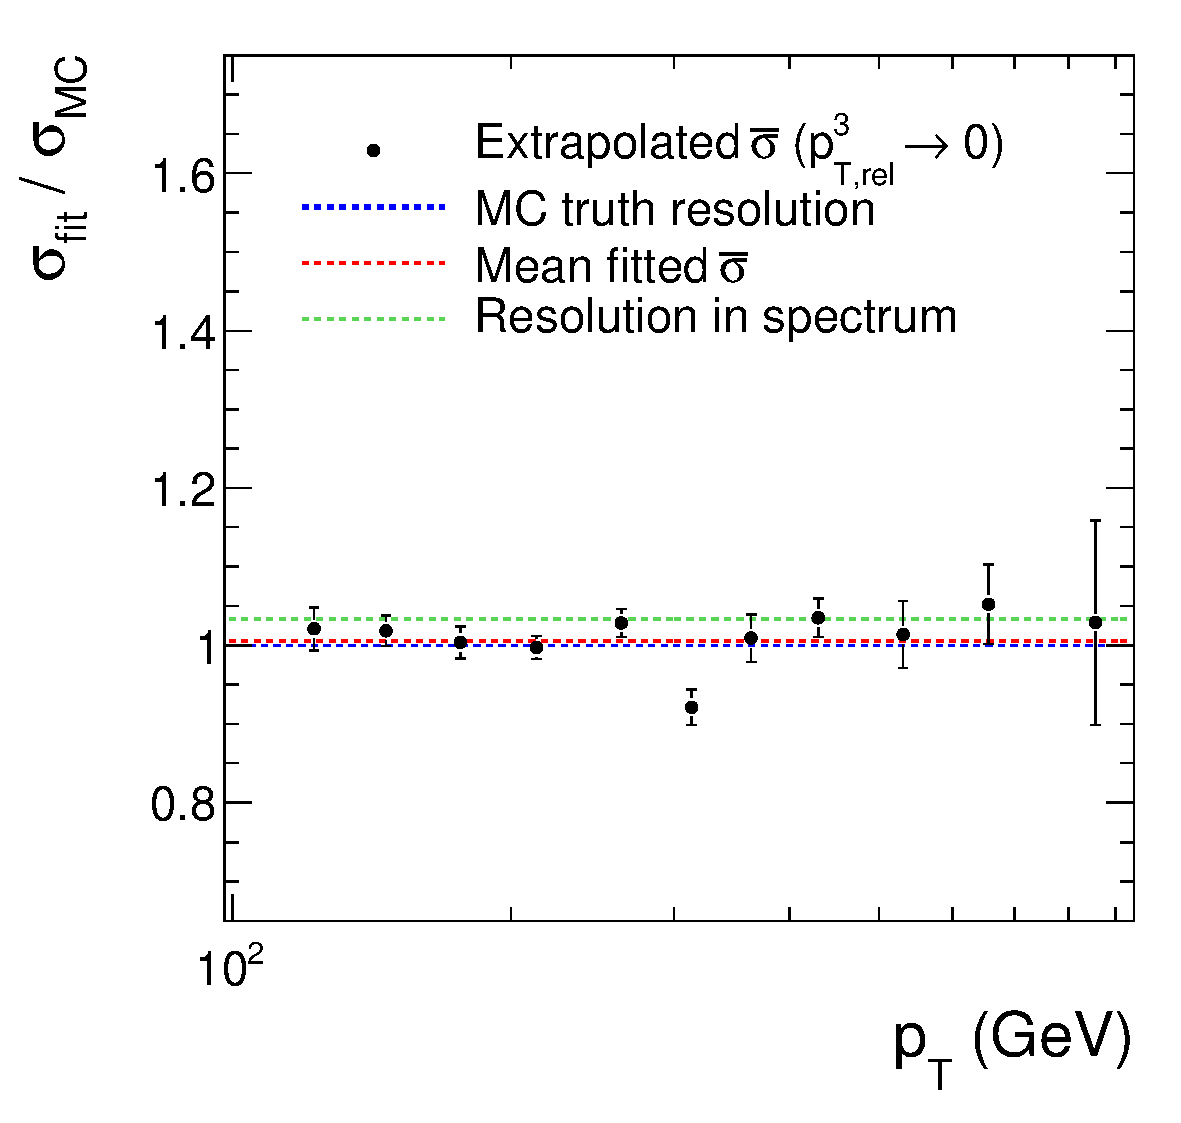
\includegraphics[width=0.3\textwidth]{figures/ResFit_Spring10QCDFlat_GaussUp30It1_Eta0_ExtrapolatedResolutionRatio} &
      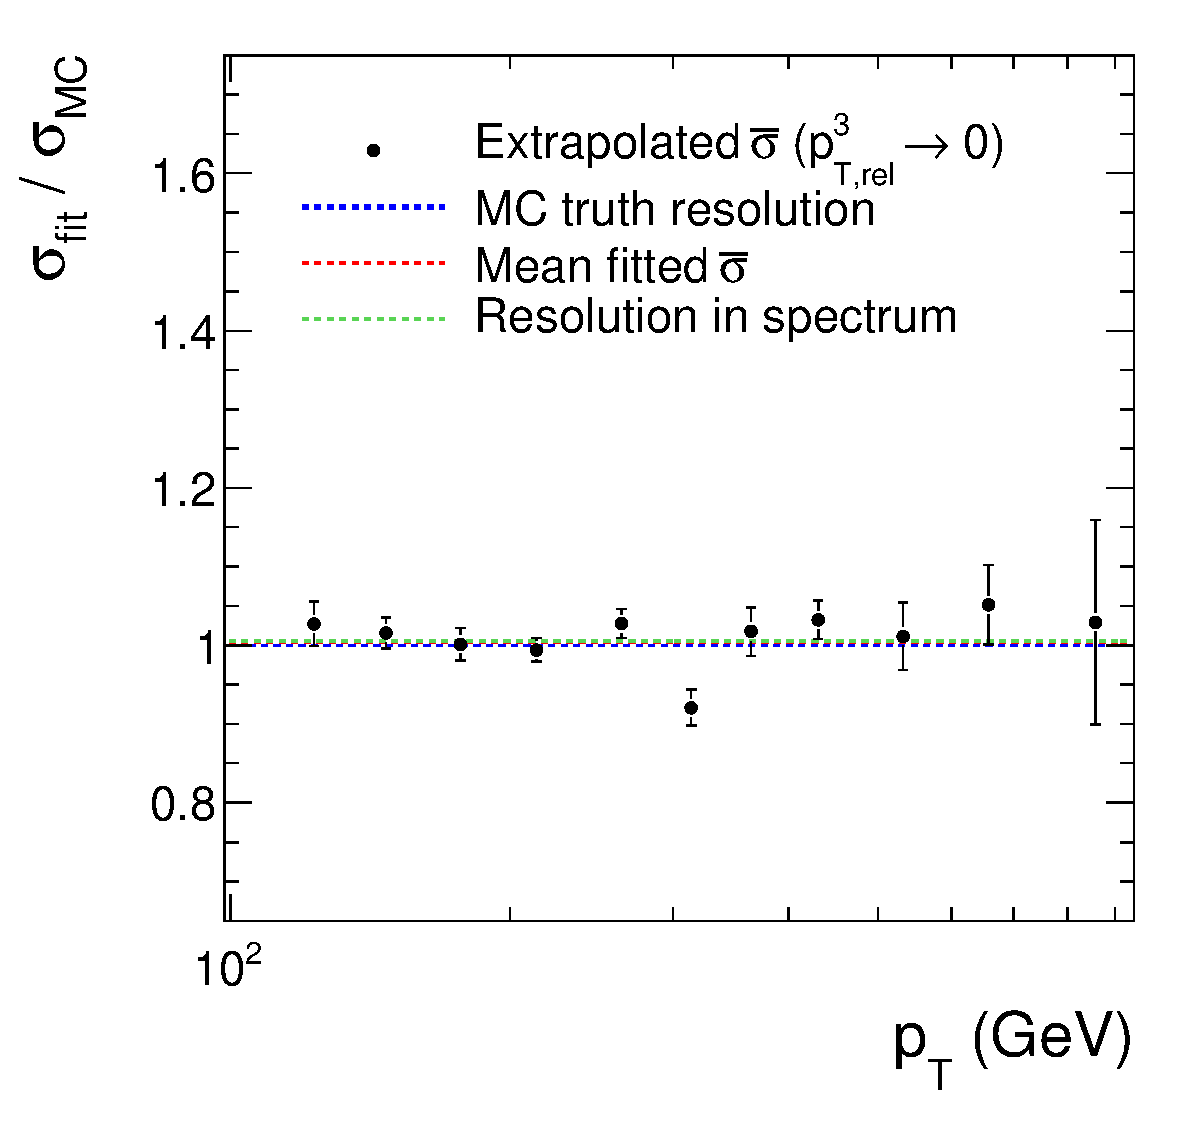
\includegraphics[width=0.3\textwidth]{figures/ResFit_Spring10QCDFlat_GaussUp30It2_Eta0_ExtrapolatedResolutionRatio}
    \end{tabular}
  \caption{The solid black markers show the measured Gaussian jet \pt resolutions in different \pt bins.
  The dashed green line is the assumed resolution to describe the selection bias during the fit.
  The dashed red line corresponds to the average measured resolution.
  Actually shown is the ratio to the Monte Carlo truth resolution in all cases.
  (\textit{Left}) The assumed resolution deviates by $30\%$ from the truth, the measured resolution by only $3.3\%$.
  (\textit{Centre}), (\textit{right}) The measured resolution from the previous iteration is taken as assumed resolution during the fit.
  The plots demonstrate the stability of an iterative procedure.}
  \label{fig:ResFig:QCD:Extrapolation:Gauss:Iterations}
\end{figure}

A description of the selection bias has been incorporated into the dijet probability density by assuming a jet \pt response $r_{0}(x|\pttrue)$ (Section~\ref{sec:ResFit:Method:Biases}).
In order to evaluate the influence of $r_{0}$ on the measured resolution, the fit has been performed with $r_{0}$ varied by $+30\%$ i.e. $\sigma_{0}\rightarrow 1.3\sigma_{0}$ (Fig.~\ref{fig:ResFig:QCD:Extrapolation:Gauss:Iterations}~\textit{left}).
The measured resolution deviates by $+(3.3 \pm 0.7)\%$ on average, demonstrating the weak influence of $r_{0}$ on the result.
A second and a third measurement have been performed, each time with the result of the previous as input for $r_{0}$, leading to decreasing average deviations (comp. Fig~\ref{fig:ResFig:QCD:Extrapolation:Gauss:Iterations} \textit{centre}, \textit{right}).
Hence, an iterative procedure is applicable. 



\subsubsection{Measurement of the full response function}\label{sec:ResFit:QCDMC:CrystalBall}

The full response function --- including non-Gaussian tails as illustrated in Fig.~\ref{fig:ResFit:QCDMC:Extrapolation:CB:ExBin:SpectrumAndMCClosure} (\textit{right}) --- is measured in different \pt bins for the central $|\eta|<1.2$ region (Table~\ref{tab:ResFit:QCDMC:Extrapolation:Binning}).
The response is parametrised with a Crystal Ball function, which consists of a Gaussian core and a powerlaw tail at the left flank:
\begin{equation*}
  r_{\bar{\sigma},\alpha,n}\left(\ptmeas|\pttrue\right) = \mathcal{N}\left\{
    \begin{array}{rl}
      \exp\left[\frac{1}{2}\left(\frac{\ptmeas-\pttrue}{\bar{\sigma}}\right)^{2}\right] & \text{if }\frac{\ptmeas-\pttrue}{\bar{\sigma}} > -\alpha \\
      A(\alpha,n)\cdot\left(B(\alpha,n) - \frac{\ptmeas-\pttrue}{\bar{\sigma}}\right)^{-n} & \text{if }\frac{\ptmeas-\pttrue}{\bar{\sigma}} \leq -\alpha
    \end{array}
  \right.\,,
\end{equation*}
where
\begin{align}
\begin{split}
  A(\alpha,n) & =  \left(\frac{n}{|\alpha|}\right)^{n}\exp\left[-\alpha^{2}/2\right] \\
      B(\alph a,n) & =  \frac{n}{|\alpha|} - |\alpha|\,.
          \end{split}	
	  \end{align}	
The function itself and	its first derivative are both continuous.
It depends on three parameters,
\begin{description}
\item[$\bar{\sigma}$] width of the Gaussian core,
\item[$\alpha$] distance in $\bar{\sigma}$ from mean of Gaussian, \pttrue, where the powerlaw tail starts,
\item[$n$] exponential in powerlaw,
\end{description}
which are measured by maximisation of the likelihood~\eqref{eq:ResFit:Likelihood}.

\begin{figure}[ht]
  \centering
  \begin{tabular}{cc}
    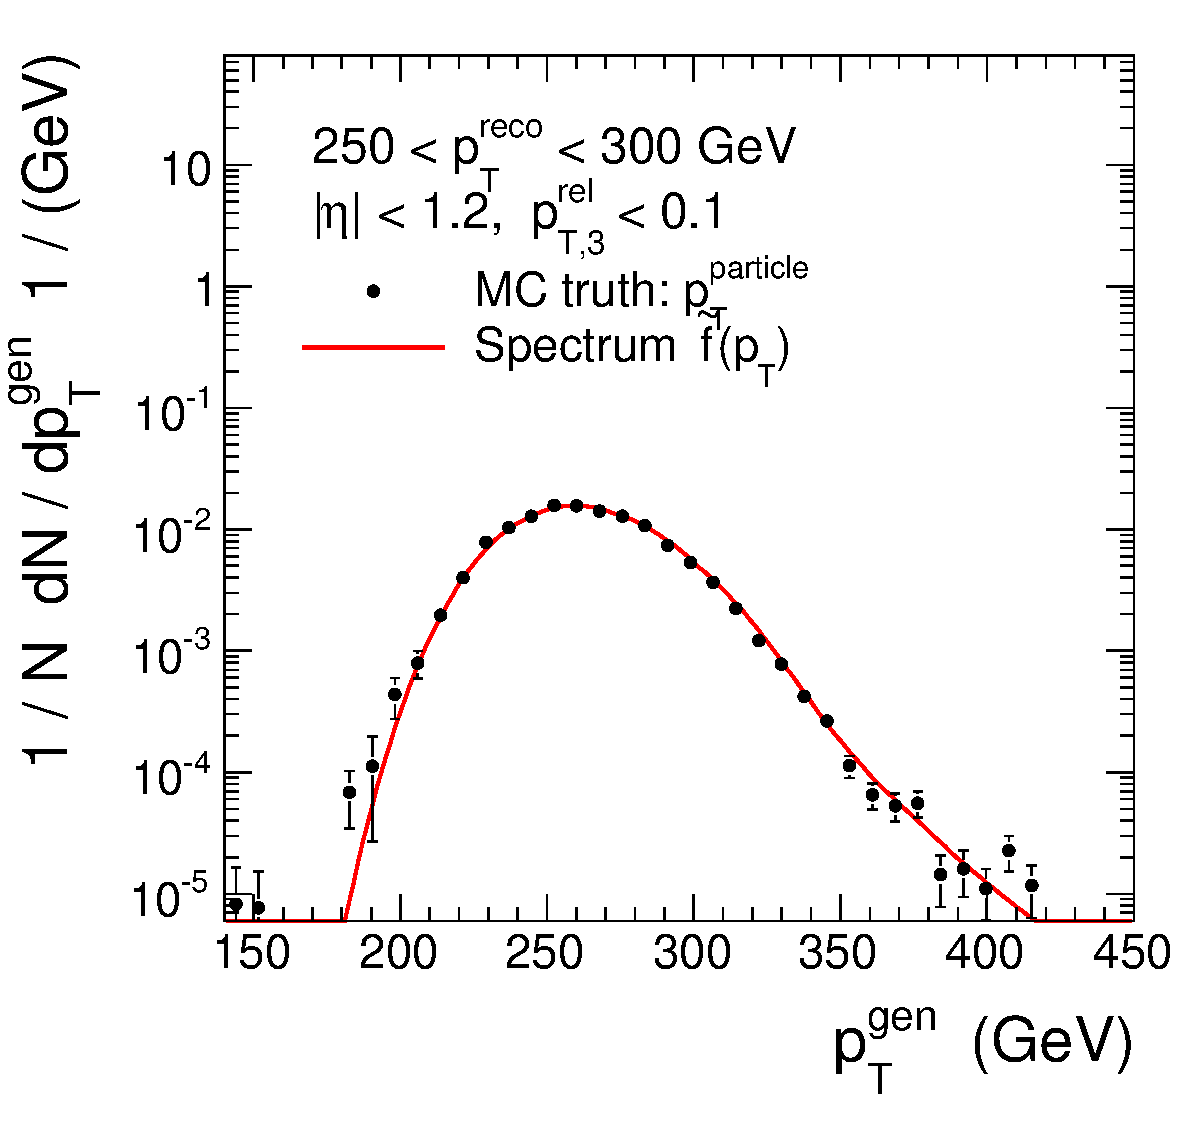
\includegraphics[width=0.45\textwidth]{figures/ResFit_Spring10QCDFlat_CB_Eta0_Spectrum_PtBin4} &
    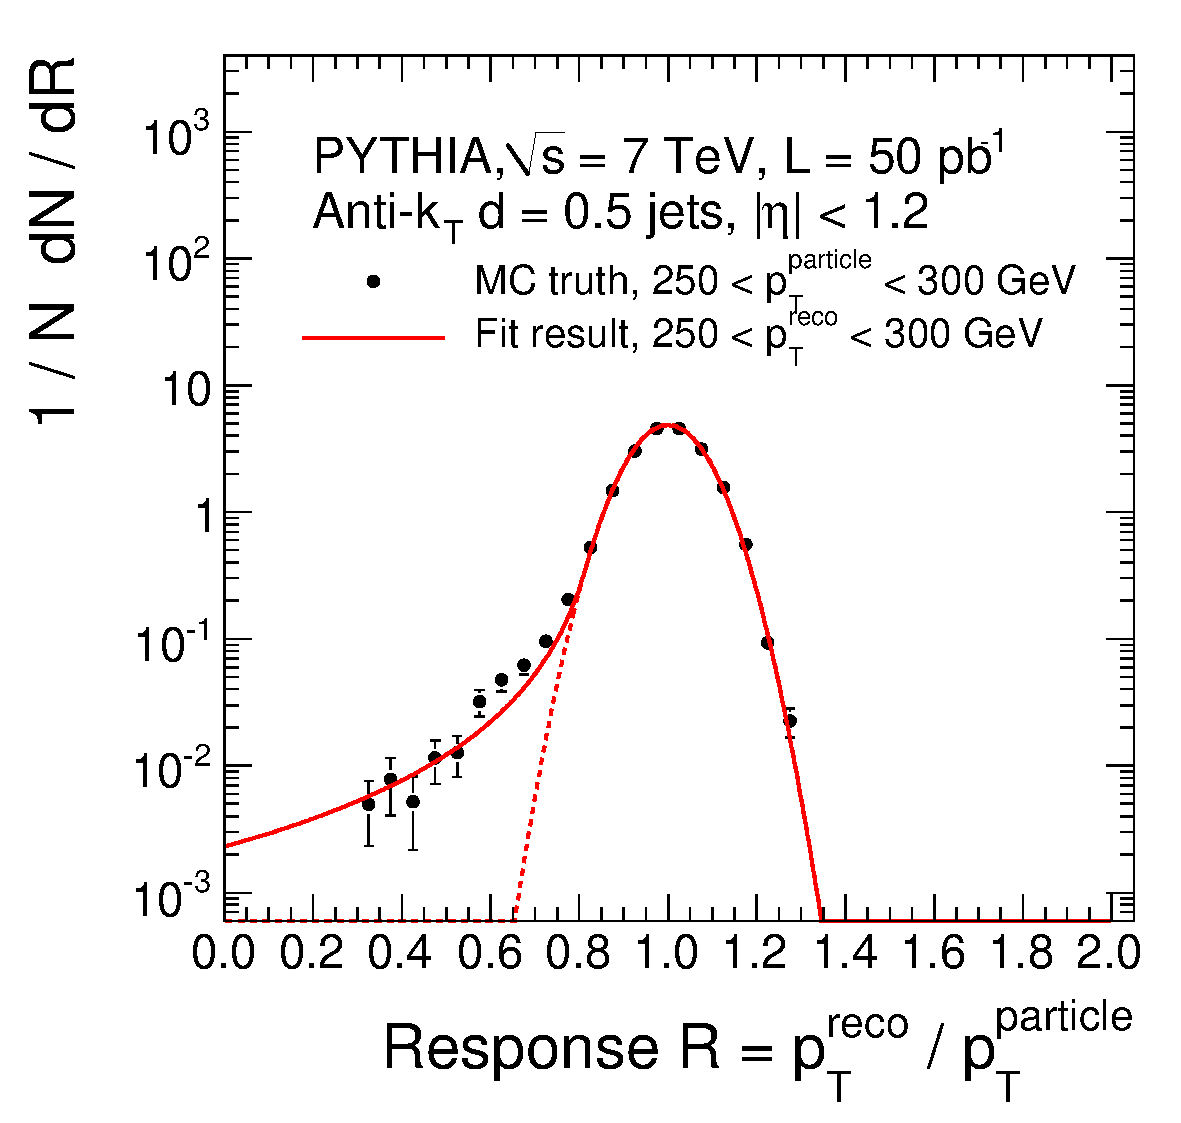
\includegraphics[width=0.45\textwidth]{figures/ResFit_Spring10QCDFlat_CB_Eta0_MCClosure_PtBin4}
  \end{tabular}
\caption{(\textit{Left}) The parametrisation of the realistic particle jet \pt spectrum in one \pt bin as used in the dijet likelihood (solid line) in comparison to the prediction from Monte Carlo truth (full circles).
  Migration effects are modelled assuming a Crystal Ball response function. 
  (\textit{Right}) Response distribution of a dijet sample selected with Monte Carlo truth information (compare the description in the text) in one \pt bin (full circles); non-Gaussian tails are visible.
  It is compared to a Crystal Ball response function (solid line) and the Gaussian core part (dashed line) evaluated with the extrapolated parameters $\bar{\sigma}$, $\alpha$, $n$ from the maximum likelihood method.}
\label{fig:ResFit:QCDMC:Extrapolation:CB:ExBin:SpectrumAndMCClosure}
\end{figure}

The parameters describing the tail, $\alpha$ and $n$, are strongly anti-correlated ($\approx95\%$).
Therefore reasonable start values are chosen (2 and 4, respectively), and the likelihood fit is iterated two times, where in the first iteration $\sigma$ and $\alpha$ are optimised while $n$ is kept fixed and in the second iteration $\sigma$ and $n$ are optimised while $\alpha$ is fixed to the previously fitted value.
In each \pt bin, again, the parameters are measured for different thresholds on \ptrel in the dijet event selection and their values are extrapolated individually to the case of $\ptrel\rightarrow0$ (Fig.~\ref{fig:ResFit:QCDMC:Extrapolation:CB:ExBin:Extrapolation}).
Note that for a proper extrapolation a set of uncorrelated parameters should be used.
However, as the Crystal Ball functional form has limited power in describing the true response distribution (see discussion below), further studies are omitted at this point.

\begin{figure}[ht]
  \centering
  \begin{tabular}{cc}
    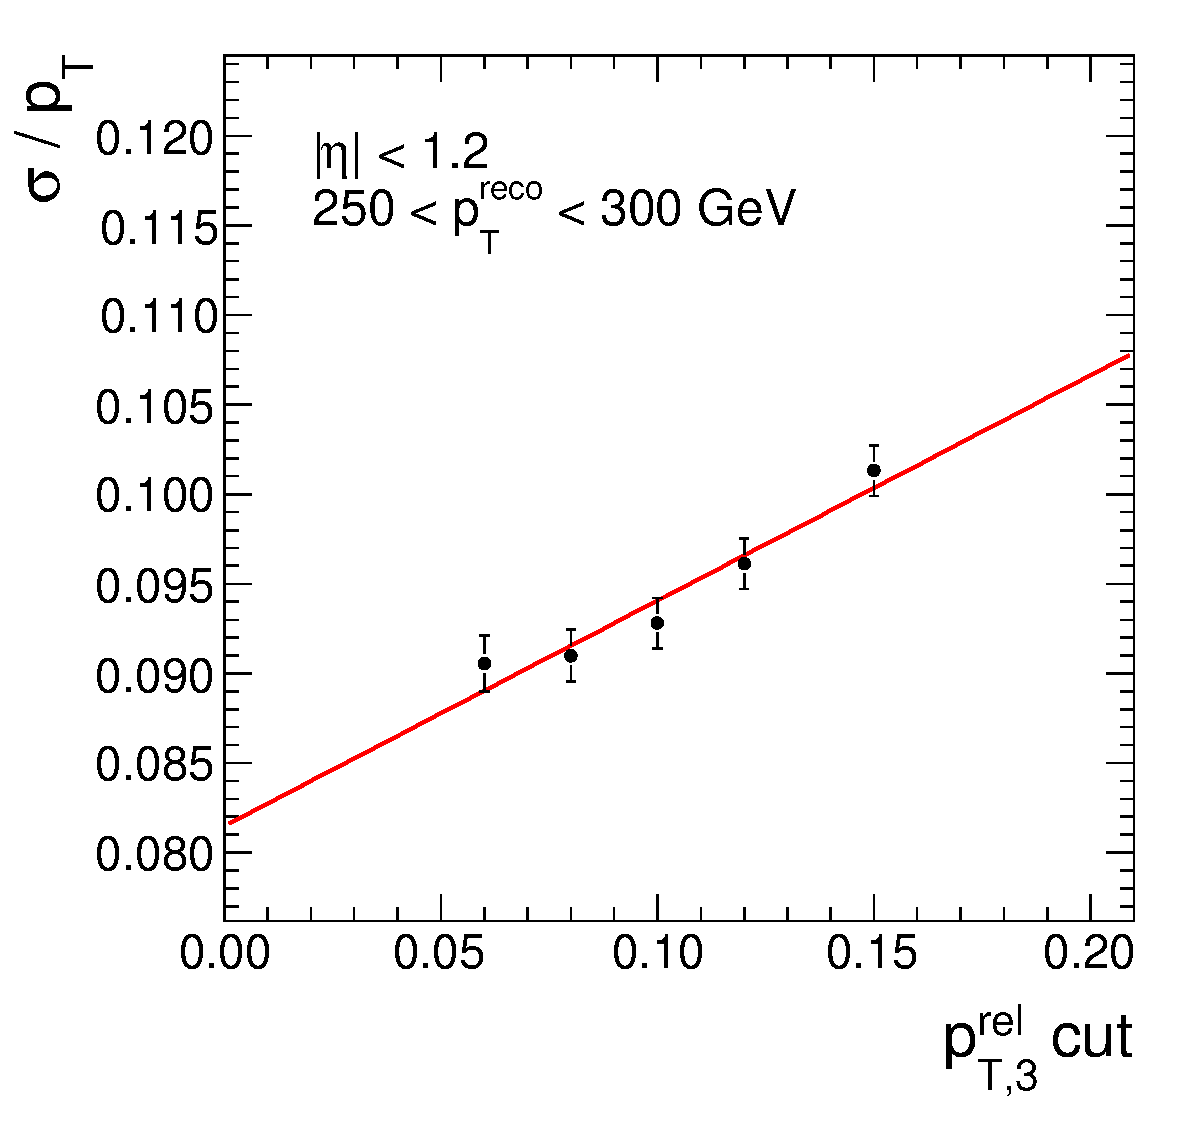
\includegraphics[width=0.45\textwidth]{figures/ResFit_Spring10QCDFlat_CB_Eta0_ExtrapolatedPar0_PtBin4} &
    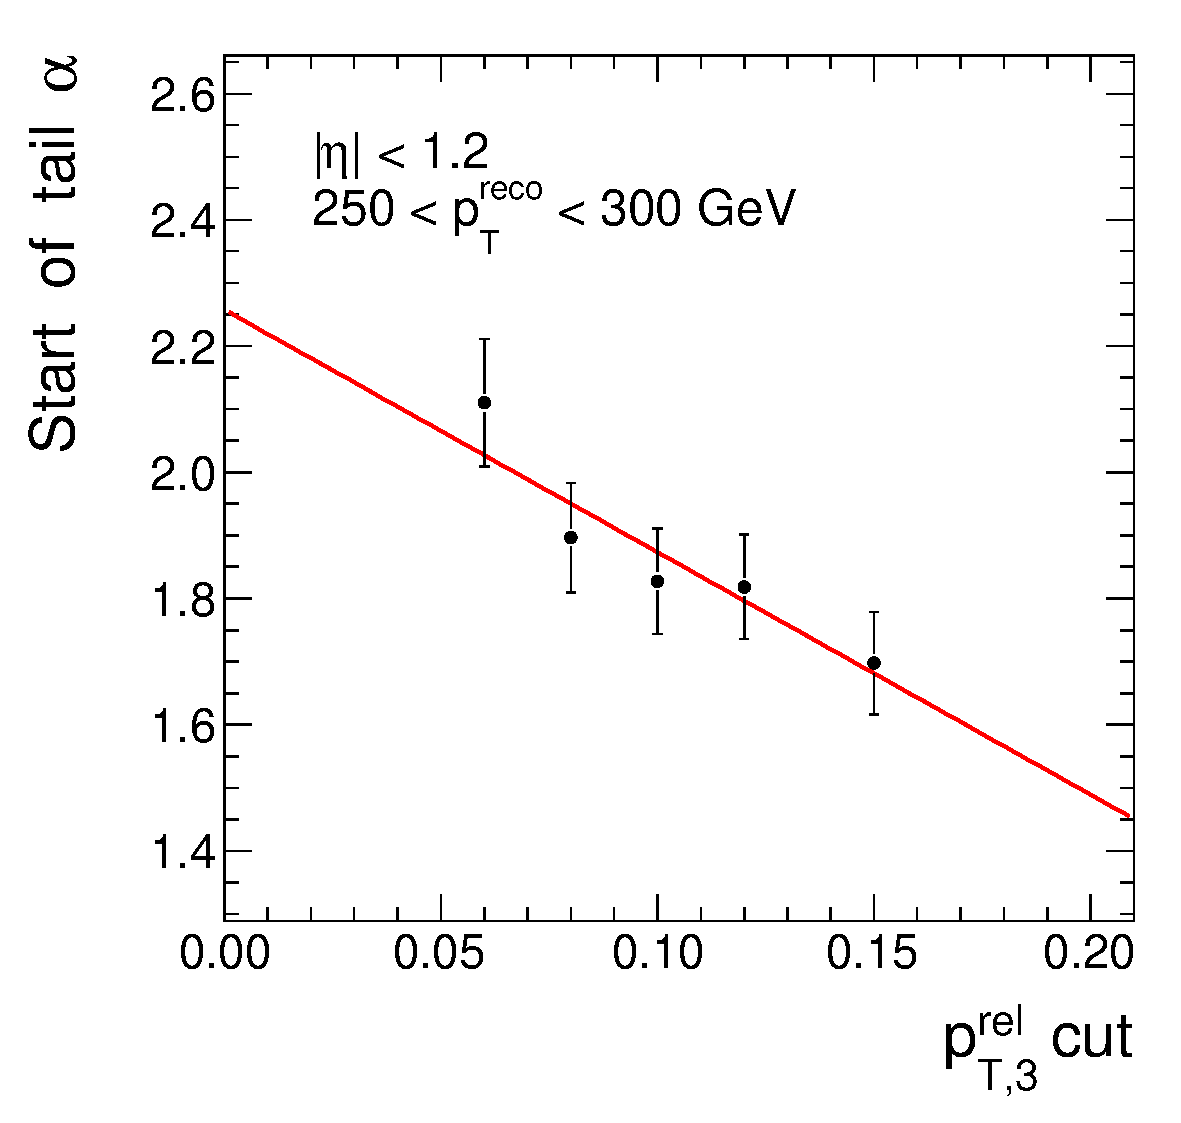
\includegraphics[width=0.45\textwidth]{figures/ResFit_Spring10QCDFlat_CB_Eta0_ExtrapolatedPar1_PtBin4} \\
    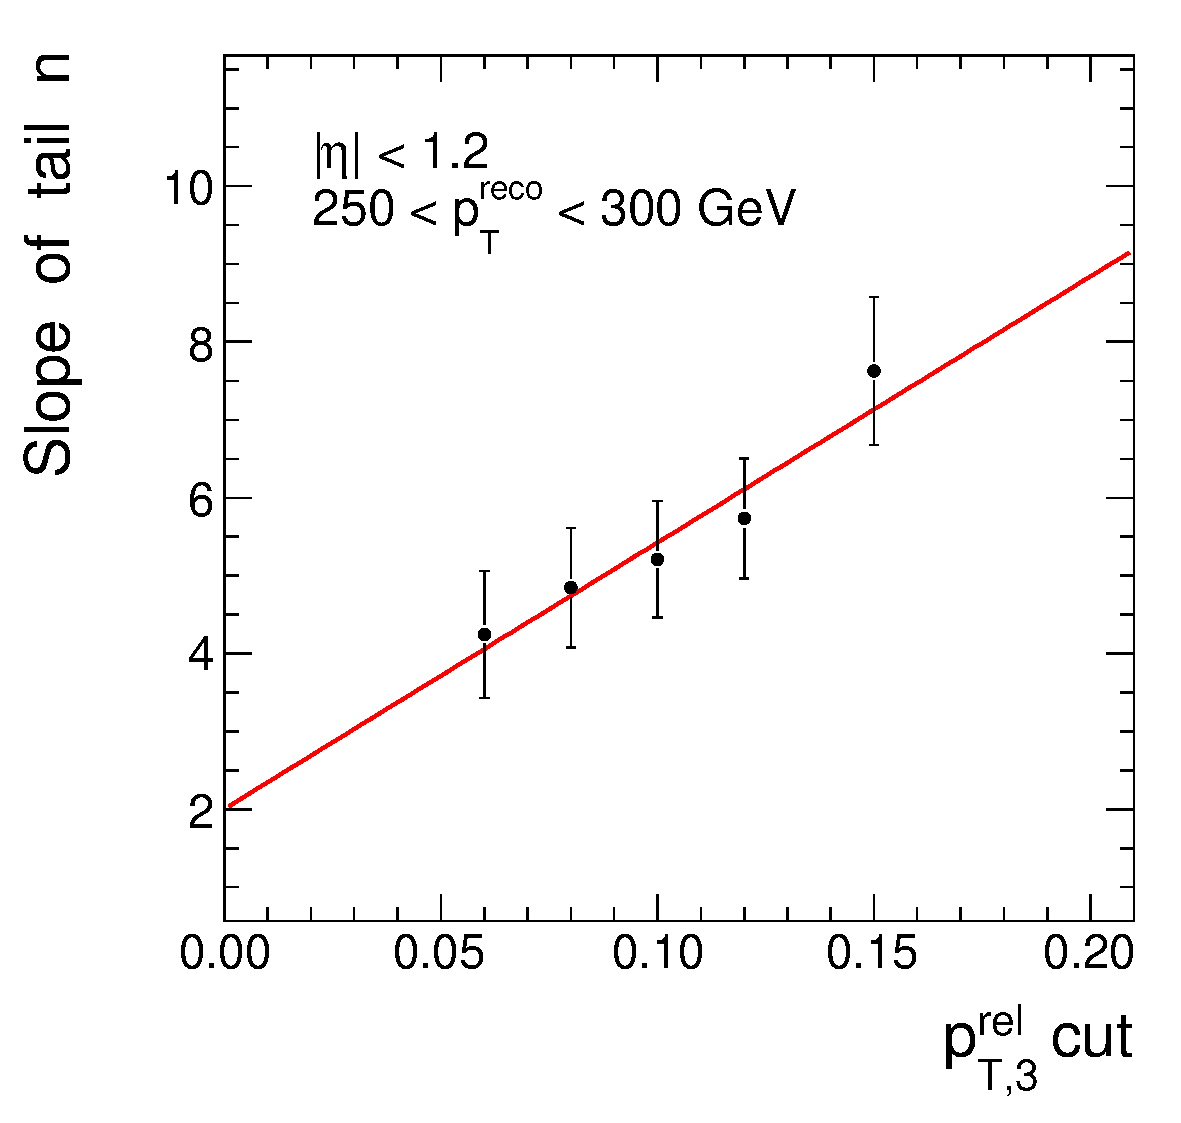
\includegraphics[width=0.45\textwidth]{figures/ResFit_Spring10QCDFlat_CB_Eta0_ExtrapolatedPar2_PtBin4} & \\
  \end{tabular}
\caption{Values of $\bar{\sigma}/\pt$ (\textit{left}), $\alpha$ (\textit{centre}), and $n$ (\textit{right}) of the Crystal Ball response function measured with the maximum likelihood method for different maximal \ptrel in the same \pt bin.
  The solid line is a linear fit to extrapolate the parameter values to the ideal case of only two jets in the final state.}
\label{fig:ResFit:QCDMC:Extrapolation:CB:ExBin:Extrapolation}
\end{figure}

Again, the selection bias (Section~\ref{sec:ResFit:Method:Biases}) is incorporated in the probability density function~\eqref{eq:ResFit:Method:ModifiedSpectrum}, where $r_{0}$ is now a Crystal Ball function.
The parameter $\sigma$ is taken from the Monte Carlo simulation as before.
For $\alpha$ and $n$ the start values 2 and 4, respectively, are used and the likelihood fit is iterated two times, where after each iteration the values of $\alpha$ and $n$ are adjusted.
(In each of the two iterations mentioned above, during which either only $\alpha$ or only $n$ is optimised, consists itself of two iterations during which the description of the spectrum is adjusted.)
The resulting assumption~$\tilde{f}(\pttrue)$ for the particle level jet \pt spectrum agrees well with the Monte Carlo truth, as demonstrated in Fig.~\ref{fig:ResFit:QCDMC:Extrapolation:CB:ExBin:SpectrumAndMCClosure} (\textit{left}) for one \pt bin (the spectra for all \pt bins are shown in Appendix~\ref{sec:ResFit:App:AllResults:CrystalBall}).

In order to validate the fit result, the response functions in each \pt bin, computed with the extrapolated parameter values, are compared to the Monte Carlo truth response distributions.
The latter are composed out of dijet events from a different selection that is based on the Monte Carlo truth information: events have been selected in bins of particle level jet \pt to avoid distortions to due migration effects.
(In contrast, the dijet events entering the fit have been selected in a data driven way and selection biases have been explicitly considered in the likelihood.)
Figure~\ref{fig:ResFit:QCDMC:Extrapolation:CB:ExBin:SpectrumAndMCClosure} (\textit{right}) shows the closure in one \pt bin, other \pt bins are shown in Appendix~\ref{sec:ResFit:App:AllResults:CrystalBall}.
The Gaussian core component of the response distribution is well described.
The measurement is also clearly sensitive to the non-Gaussian component of the response distribution and the tail is reasonably well described by the Crystal Ball powerlaw tail.
However, the structure of the Monte Carlo truth distribution features more structure than a simple monotonic decrease of the same curvature which can consequently not be modelled by the Crystal Ball function.
